\appendix

\chapter{Installation Guidelines}

\subsection{Mandatory Steps for preparing the environment}
In order to successfully replicate the implementation in your environment some prior information is needed. First of all, we strongly encourage to install HLF in an AMD processor based computer since HLF does not support ARM architectures. However uploading code to Esp Eye it does not matter from which OS you are using. Throughout this guideline it is assumed that Git is installed. 

\subsection{Arduino Firmware for Esp Eye}

All the files for the Esp Eye, IoT Gateway and HLF reside in the shared git repository. To start with use the command below in you desired directory where you want to start replicating this project. 


\framebox[1.1\width]{git clone https://github.com/eesati/Master-Thesis.git } \par

After having done the above there are a number of directories, the ones which we are interested now is the {\fontfamily{ccr}\selectfont Arduino} folder and {\fontfamily{ccr}\selectfont Arduino15} folder. In order to upload firmware Arduino Ide must be installed. 
In order to do so follow this link for installation depending on your environment 
\framebox[1.1\width]{ https://www.arduino.cc/en/Guide}

In order to program Esp Eye with Arduino IDE the ESP32 board needs to be installed by following these steps: 
\begin{enumerate}
    \item In Arduino, go to File> Preferences
    \item Paste the following link \framebox[1.1\width]{ https://dl.espressif.com/dl/package\_esp32\_index.json} under Additional Boards Manager and click OK.
    
    
    \begin{figure}[!htb]
    \centering
    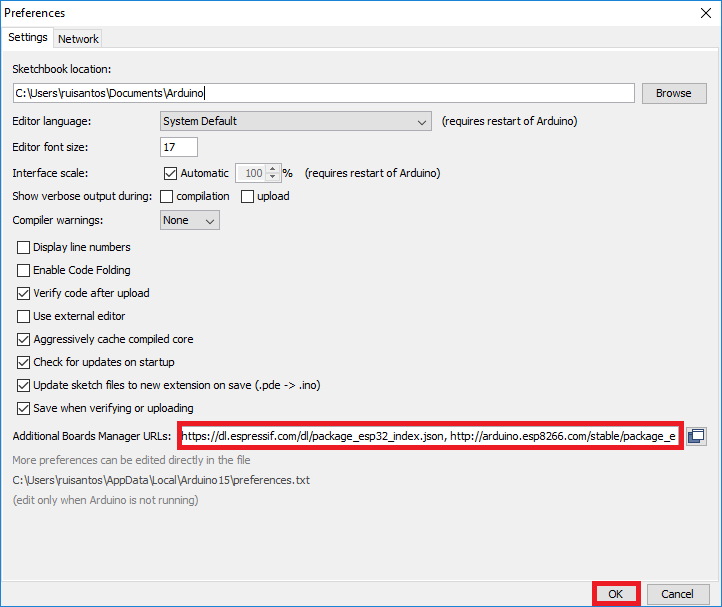
\includegraphics[width=1\textwidth]{figures/ArduinoIDE.png}
    \caption{Installing ESP32 board.}
    \label{fig:eessdff}
\end{figure}
    \item After that Go to Tools > Board > Boards Manager… and search for esp32 and install the latest version of it. See Figure~\ref{fig:eessdff}. 
    
      \begin{figure}[!htb]
    \centering
    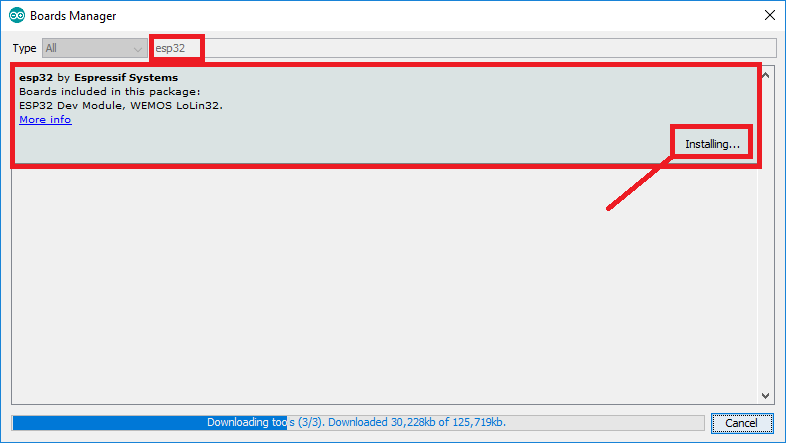
\includegraphics[width=1\textwidth]{figures/Arduinoboard.png}
    \caption{Installing ESP32 library.}
    \label{fig:eessdff}
\end{figure}
    \item It should be done. Now you can go to Tools > Board and select AI THINKER. 

 
\end{enumerate}


After that a number of libraries have to be installed in Arduino IDE: {\fontfamily{ccr}\selectfont Arduino\_JSON}, {\fontfamily{ccr}\selectfont Wifi}, {\fontfamily{ccr}\selectfont Wifi101}, {\fontfamily{ccr}\selectfont ESP32\_Mail\_Client} and {\fontfamily{ccr}\selectfont NTPClient}. 
By going to Tools > Manage Libraries you can install each one by one. 

The {\fontfamily{ccr}\selectfont Arduino} folder contains the firmware for Esp Eye and additional libraries. There are multiple Arduino files which show the step by step implementation. The last file to be uploaded in Arduino is: 

\framebox[1.1\width]{ Arduino/Final\_for\_submission/Final\_for\_submission.ino  } \par

\subsubsection{Registering Face IDs}
However in order to register face ids there is another sketch that needs to be uploaded to do that. Since the face ids are stored in flash then some changes need to be done in installation folder where Arduino IDE is installed in your computer. Before uploading the code for registration of faces there is a need to partition the flash to save little space for face Ids. Now you need to go to the partition folder which is typically located under this directory:
 
For windows downloaded Arduino Ide from Arduino Website:

\framebox{\parbox{\linewidth-2}{\itshape%
  C > Users > *your-user-name* > AppData > Local > Arduino15  > packages > esp32 > hardware > esp32 > 1.0.4 > tools > partitions }}
 

For Mac or Linux: 

\framebox{\parbox{\linewidth-2}{\itshape%
  Users > *your-user-name* > Library > Arduino15  > packages > esp32 > hardware > esp32 > 1.0.4 > tools > partitions }}

Now copy the file {\fontfamily{ccr}\selectfont faceid\_partitions.csv} found in the root directory of the repository and paste in the directory above. 

Now to let the board know about the partitioning there is a need to update the file {\fontfamily{ccr}\selectfont board.txt } located under the folder 1.0.4 which is in the two directories back from the partition folder and add the following lines: 

\framebox{\parbox{\linewidth-2}{\itshape%
esp32wrover.menu.PartitionScheme.faceid\_partition=Face Recognition (2621440 bytes with OTA)\par
esp32wrover.menu.PartitionScheme.faceid\_partition.build.partitions=faceid\_partitions

esp32wrover.menu.PartitionScheme.faceid\_partition.upload.maximum_size=2621440}}

Now use the {\fontfamily{ccr}\selectfont Enroll\_faces.ino } sketch to enroll face ids. After enrolling faces then upload the {\fontfamily{ccr}\selectfont Final\_for\_submission.ino } sketch. Finally, since the Esp Eye firmware acts as a station there is a need to update the SSID and password to connect to. 



\subsection{Hyperledger Fabric installation}

The Fabric network with implemented chaincode is located under {\fontfamily{ccr}\selectfont HLF } directory. At the time when we installed it HLF was the latest version but now it is no longer anymore and it is known as v2.1. 

We strongly encourage to have a look at the official HLB site for installation guidelines located at :

\framebox{\parbox{\linewidth-2}{\itshape%
https://hyperledger-fabric.readthedocs.io/en/release-2.1/getting\_started.html}}

\subsubsection{Prerequisites}
Before beginning the installation, there a number of prerequisites that need to be followed. Which can be seen also here in the link below:

\framebox{\parbox{\linewidth-2}{\itshape%
https://hyperledger-fabric.readthedocs.io/en/release-2.1/prereqs.html}}


\begin{enumerate}
    \item  The latest version of git for your OS
    \item The latest version of cURL
    \item The latest version of Docker and Docker Compose
\end{enumerate}

\subsubsection{Installing Hyperledger Fabric binaries and docker images}

\subsubsection{First method}
Now it is time to install Hyperledger Fabric binaries and docker images. For now there are two ways to do that, one way is to install a clean copy of HLP. Which can be seen in more detail in this link : 

\framebox{\parbox{\linewidth-2}{\itshape%
https://hyperledger-fabric.readthedocs.io/en/release-2.1/install.html}}

The github repository for HLF need to be cloned in a local directory, for macOS it has to use a location under /Users:

\framebox{\parbox{\linewidth-2}{\itshape%
git clone https://github.com/hyperledger/fabric-samples.git }}

Now it is the time to install binaries and docker images. To do so there should be a fabric-sample directory. In terminal under that directory execute the following command: 

\framebox{\parbox{\linewidth-2}{\itshape%
curl -sSL https://bit.ly/2ysbOFE | bash -s -- <fabric\_version> <fabric-ca\_version> <thirdparty\_version> }}



Which in our case would translate to v2.1 as below: 

\framebox{\parbox{\linewidth-2}{\itshape%
curl -sSL https://bit.ly/2ysbOFE | bash -s -- 2.1.1 1.4.7 0.4.20 }}


To pick up the docker containers without going to the path for each binary, it is recommended to do this: 

\framebox{\parbox{\linewidth-2}{\itshape%
export PATH=<path to the cloned HLF location>/bin:$PATH

}}




After that copy the {\fontfamily{ccr}\selectfont imagestore} folder under HLF and paste at the cloned copy of the Hyperledger Fabric. Under {\fontfamily{ccr}\selectfont chaincode} folder of HLF  we have the chaincode with a folder named imagestore copy that and paste under chaincode of the newly cloned Hyperledger Fabric under chaincode. It should by now be ready to run the project. 




\subsubsection{Second method}
The second way is to use the HLF directory of ours but a number of changes need to be done. First the {\fontfamily{ccr}\selectfont bin} folder has to be deleted because it contains the previous installed docker images. 

After that the binaries and docker images need to be installed locally. Similarly as above under the HLF directory the binaries need to be installed using the following command in Terminal: 

\framebox{\parbox{\linewidth-2}{\itshape%
curl -sSL https://bit.ly/2ysbOFE | bash -s -- 2.1.1 1.4.7 0.4.20 }}


To pick up the docker containers without going to the path for each binary, it is recommended to do this: 

\framebox{\parbox{\linewidth-2}{\itshape%
export PATH=<path to the cloned HLF location>/bin:$PATH

}} 
It is now expected that Hyperledger Fabric is installed and ready to be used. The two methods apply to all OS however the prerequisites may have to be installed using different package manager. 
For any issues it is recommended to follow the official HLF documentation links as above.





\subsubsection{Hyperledger Fabric application SDKs} 

Hyperledger Fabric provides a number of SDKs to support developing applications. Since we are using nodejs for the server, similarly nodejs SDK for fabric client is used. 
The prerequisites for nodejs SDK is that the following must be installed first: 

\begin{itemize}
    \item Node.js, version 10 is supported from 10.15.3 and higher
    \item  Node.js, version 12 is supported from 12.13.1 and higher
    \item npm tool version 6 or higher
\end{itemize}

To install the nodejs SDK:

\framebox{\parbox{\linewidth-2}{\itshape% 
npm install fabric-network
}} 

Hyperledger Fabric also offers a contract API for developing smart contacts. For nodejs use following command to install it:  

\framebox{\parbox{\linewidth-2}{\itshape% 
npm install --save fabric-contract-api
}} 

The main folders where our implementation lies in the source code of our project is {\fontfamily{ccr}\selectfont imagestore} folder. We strongly recommend to do :

\framebox{\parbox{\linewidth-2}{\itshape% 
npm install
}} 
under the folder
{\fontfamily{ccr}\selectfont /imagestore/javascript} where the nodejs server and HLF client are and under {\fontfamily{ccr}\selectfont /imagestore/frontend} which is the react web application.  


\subsubsection{Running Hyperledger Fabric}
To start the Fabric network, docker must be running. 
To start with in Terminal go to {\fontfamily{ccr}\selectfont imagestore} and do: 

\framebox{\parbox{\linewidth-2}{\itshape% 
./startNetwork.sh javascript
}}
And it should look like the Figure Figure~\ref{fig:eessdffsfsf}.

    \begin{figure}[!htb]
    \centering
    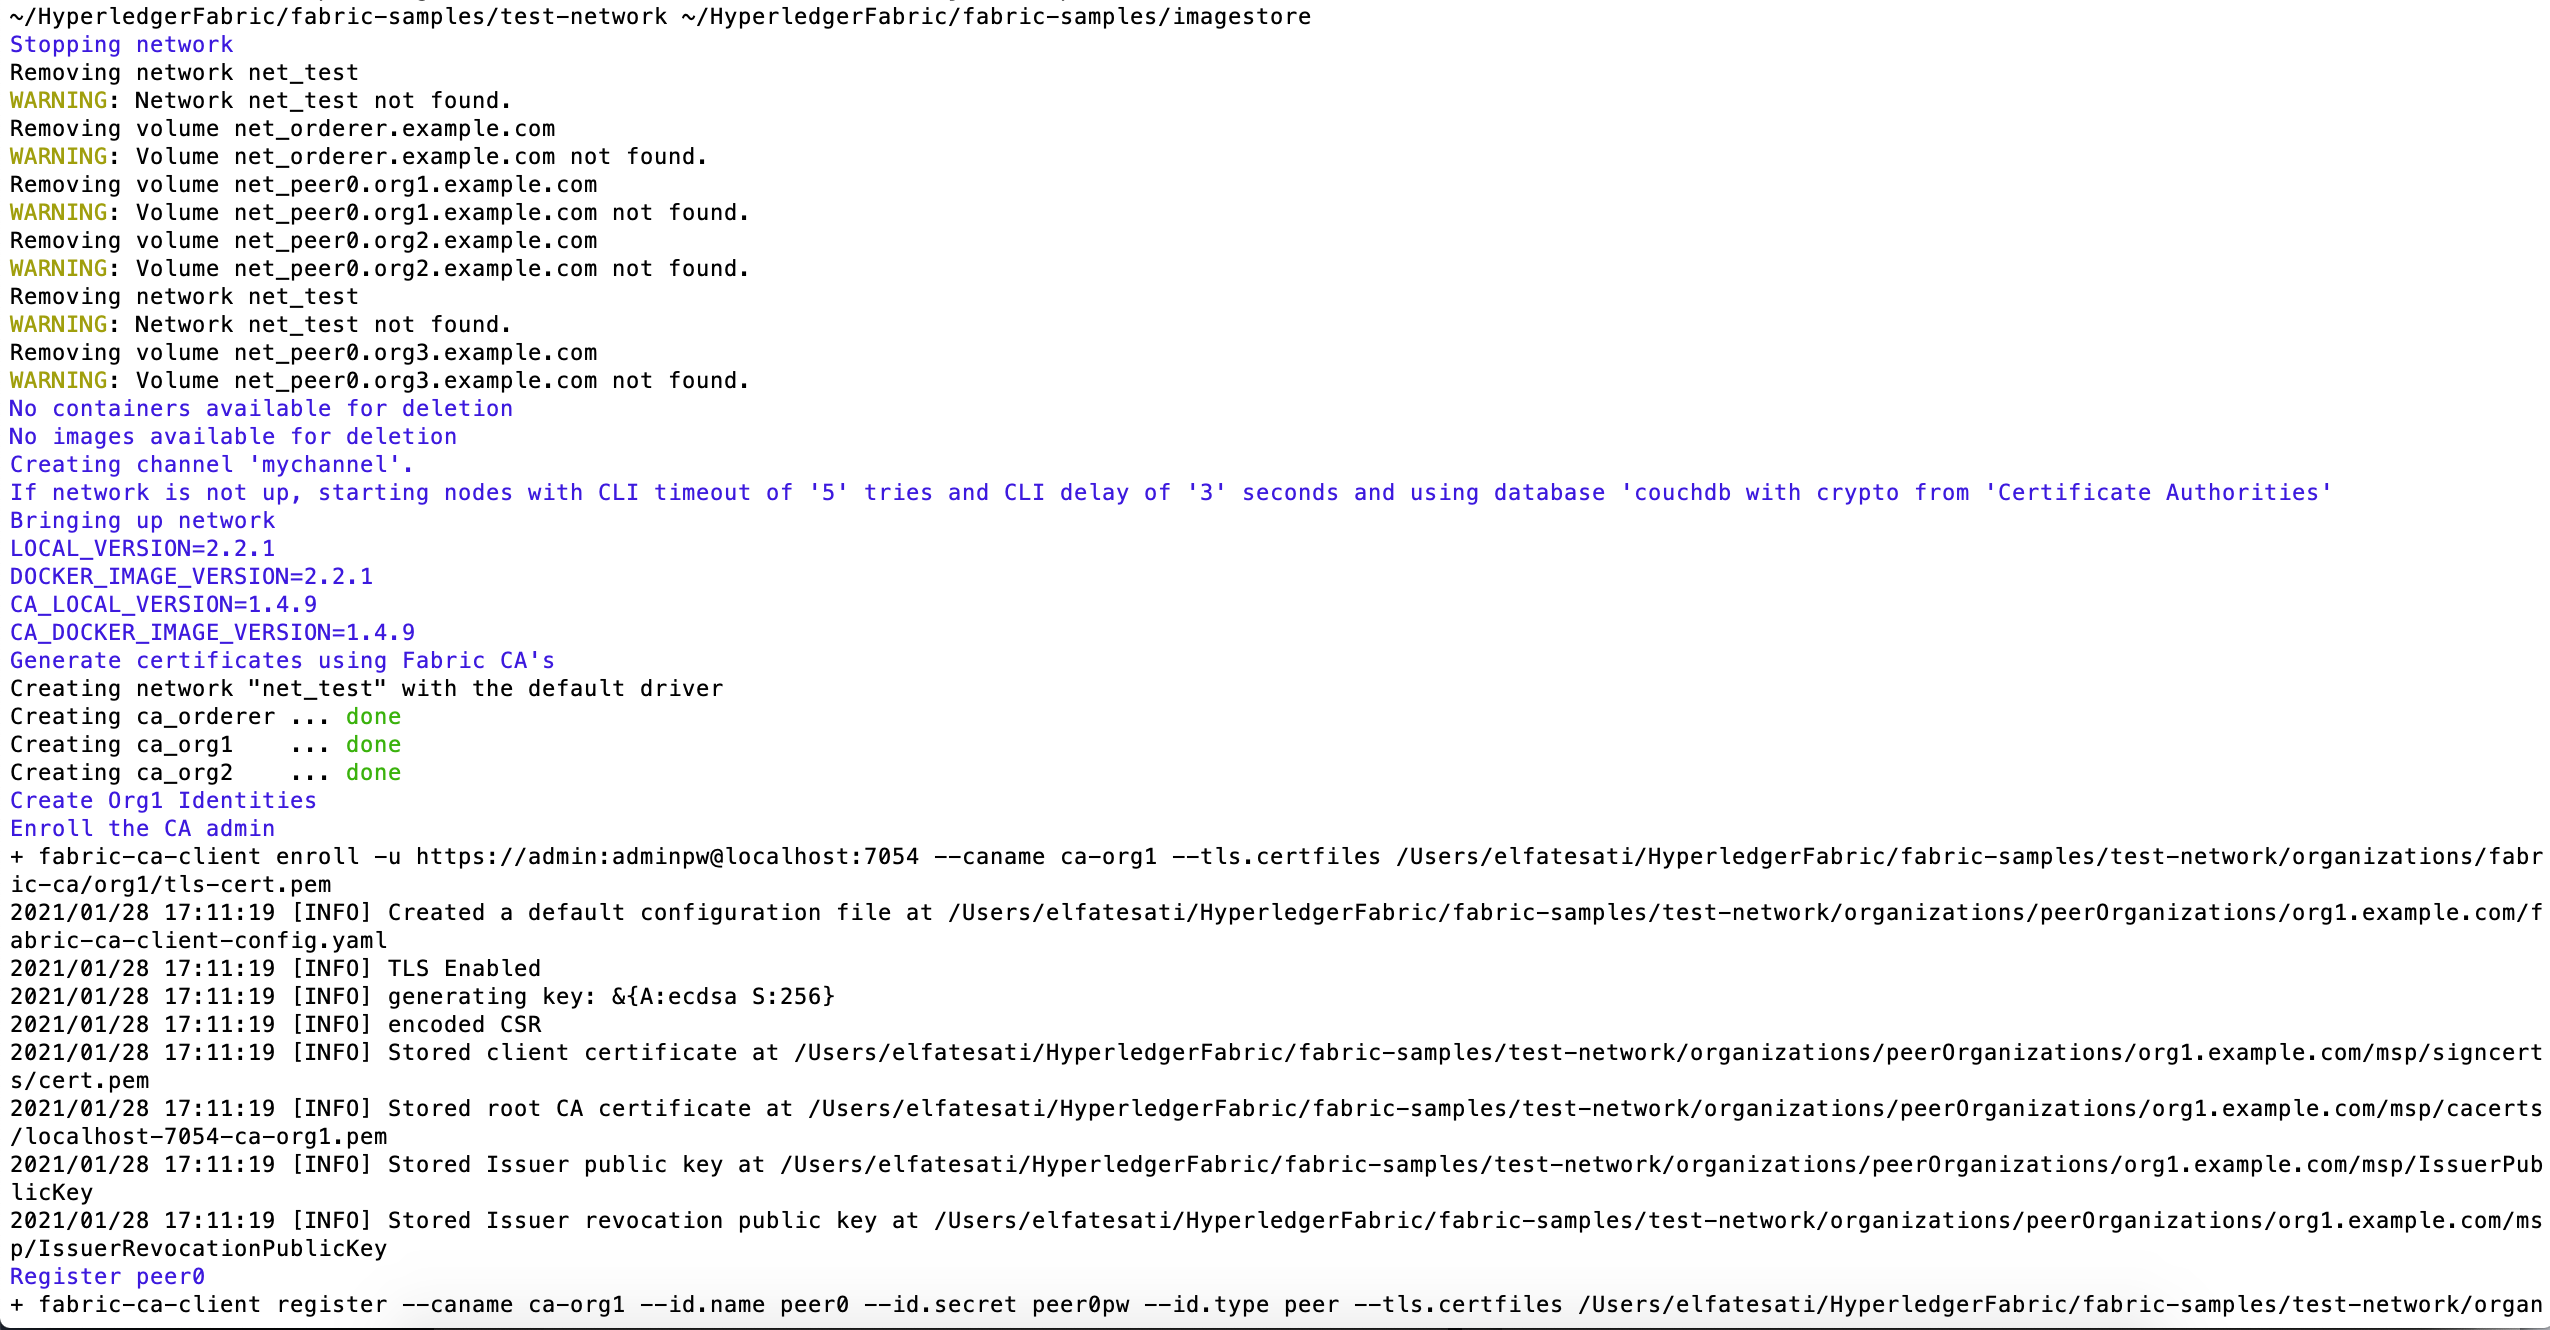
\includegraphics[width=1\textwidth]{figures/RunningHLF.png}
    \caption{ }
    \label{fig:eessdffsfsf}
\end{figure}
This script will start the network and docker containers, besides it will simultaneously deploy the smart contract specified in the chaincode. If you want to know more see the startNetwork.sh file. Basically it creates the network with 2 organisations and 2 ordering peers. The chaincode also gets deployed which is located under 
{\fontfamily{ccr}\selectfont /chaincode/imagestore/javascript/}.

The last step wow to create an Administrator and a user move to {\fontfamily{ccr}\selectfont /imagestore/javascript/} and run: 

\framebox{\parbox{\linewidth-2}{\itshape% 
node enrollAdmin.js
}}

\framebox{\parbox{\linewidth-2}{\itshape% 
node registerUser.js
}}


\subsection{Running the Web Application}

The web application is located under {\fontfamily{ccr}\selectfont /imagestore/frontnend}, cd into this folder and do : 
\framebox{\parbox{\linewidth-2}{\itshape% 
npm install
}}
\framebox{\parbox{\linewidth-2}{\itshape% 
npm start
}}

\subsection{Fabric Explorer}
Fabric Explorer is optional. To install it you can use the following link and it offers a number of options: 

\framebox{\parbox{\linewidth-2}{\itshape% 
https://github.com/hyperledger/blockchain-explorer
}}

We recommend installing it using docker. The Fabric Explorer container comes automatically when binaries are installed . First of all it assumes the Fabric network is already running. Under the root directory of the source of this project there is a folder named {\fontfamily{ccr}\selectfont Fabricexplorer} which holds the necessary files to make Explorer running. The file that should be updated is the {\fontfamily{ccr}\selectfont connection-profile/test-network.json}. In this file the {\fontfamily{ccr}\selectfont adminPrivateKey} has to be updated with the newly generated private key with location in Hyperledger Fabric: 



\framebox{\parbox{\linewidth-2}{\itshape% 
/peerOrganizations/org1.example.com/users/Admin@org1.example.com/msp/keystore
}}



\chapter{Contents of the CD}
The CD contains the following:

\begin{itemize}
    \item a folder with the Arduino source code
    \item a folder with the Arduino Libraries
    \item a folder for Hyperledger Fabric
    \item a folder with Web Application
    \item a folder with R Code
    \item a folder with Fabric Explorer
    \item a folder with the thesis source code and the final thesis pdf
 
\end{itemize}

\emph{All contents of the CD are available online on my GitHuB \url{https://github.com/eesati/Master-thesis}}




%\section{C-RAN for LoRa}\label{c-ran-for-lora}

An Arduino with a LoRa shield sends out packets over the air in an
interval. Some packets require an acknowledgment (ACK). If an ACK is
required, the Arduino waits for a certain amount of time for the ACK. If
the ACK arrives in time, the Arduino starts transmitting the next
packet. If not, the Arduino will resend the packet and again wait for
the ACK.

The RRH (Remote Radio Head) receives radio waves with a LimeSDR. The RRH
streams the IQ samples over the network the the BBU (Base Band Unit).

The BBU decodes the message. If the message says it require and ACK, the
BBU send out IQ samples of the ACK message over the network to the RRH
which transmits them back over the air to the Arduino.

\subsection{Run with Docker}\label{run-with-docker}

\begin{enumerate}
\def\labelenumi{\arabic{enumi}.}
\tightlist
\item
  Clone the repo
\item
  Go to the docker directory
\end{enumerate}

\subsubsection{\texorpdfstring{\textbf{\emph{Info}}}{Info}}\label{info}

\begin{itemize}
\tightlist
\item
  The container run in priviledged mode to easily access plugged in USB
  devices
\item
  The container run in network mode host (No NAT or Bridge has to be
  considered). This means the containers have the ip address of the host
  machine. If RRH and BBU run on different machines, find out their
  respective IP with \emph{ifconfig} and pass the address as arguments
  in the docker-compose.yml, see below.
\end{itemize}

\begin{center}\rule{0.5\linewidth}{\linethickness}\end{center}

\subsection{RRH}\label{rrh}

In the RRH directory run:

\begin{verbatim}
docker-compose up 
\end{verbatim}

This starts the Remote Radio Head. The RRH looks for a LimeSDR, it
prints errors if it cannot find one. You can plug one in after the
container has started and it should get detectet. By default it uses the
first LimeSDR it can find.

\subsubsection{Parameters}\label{parameters}

There are various parameters which you can specify in the
\emph{docker-compose.yml} file.

Run this to see what the possible params are:

\begin{verbatim}
./zero_mq_split_a.py -h
\end{verbatim}

Output:

\begin{verbatim}
Usage: zero_mq_split_a.py: [options]

Options:
  -h, --help            show this help message and exit
  --RX-device-serial=RX_DEVICE_SERIAL
                        Set RX_device_serial [default=]
  --TX-device-serial=TX_DEVICE_SERIAL
                        Set TX_device_serial [default=]
  --capture-freq=CAPTURE_FREQ
                        Set capture_freq [default=868.5M]
  --samp-rate=SAMP_RATE
                        Set samp_rate [default=1.0M]
  --zmq-address-iq-in=ZMQ_ADDRESS_IQ_IN
                        Set zmq_address_iq_in [default=tcp://127.0.0.1:5052]
  --zmq-address-iq-out=ZMQ_ADDRESS_IQ_OUT
                        Set zmq_address_iq_out [default=tcp://*:5051]
\end{verbatim}

\begin{longtable}[]{@{}ll@{}}
\toprule
\begin{minipage}[b]{0.18\columnwidth}\raggedright\strut
Param\strut
\end{minipage} & \begin{minipage}[b]{0.18\columnwidth}\raggedright\strut
Explanation\strut
\end{minipage}\tabularnewline
\midrule
\endhead
\begin{minipage}[t]{0.18\columnwidth}\raggedright\strut
RX-device-serial\strut
\end{minipage} & \begin{minipage}[t]{0.18\columnwidth}\raggedright\strut
By default, the program will use the first LimeSDR it can find for
receiving and transmitting signal. If you have two devices you can
specify which should receive by passing the device Serial (See section
\textbf{Help} for more info)\strut
\end{minipage}\tabularnewline
\begin{minipage}[t]{0.18\columnwidth}\raggedright\strut
TX-device-serial\strut
\end{minipage} & \begin{minipage}[t]{0.18\columnwidth}\raggedright\strut
By default, the program will use the first LimeSDR it can find for
receiving and transmitting signal. If you have two devices you can
specify which should transmit by passing the device Serial (See section
\textbf{Help} for more info)\strut
\end{minipage}\tabularnewline
\begin{minipage}[t]{0.18\columnwidth}\raggedright\strut
capture-freq\strut
\end{minipage} & \begin{minipage}[t]{0.18\columnwidth}\raggedright\strut
The frequency in Hz at which the RRH listens for signals. Default value
is 86850000\strut
\end{minipage}\tabularnewline
\begin{minipage}[t]{0.18\columnwidth}\raggedright\strut
samp-rate\strut
\end{minipage} & \begin{minipage}[t]{0.18\columnwidth}\raggedright\strut
How many samples per second. Default value is 1000000. Must be at least
double the bandwidth of the expected signal see \emph{Nyquist-Shannon
principle}\strut
\end{minipage}\tabularnewline
\begin{minipage}[t]{0.18\columnwidth}\raggedright\strut
zmq-address-iq-in\strut
\end{minipage} & \begin{minipage}[t]{0.18\columnwidth}\raggedright\strut
ZMQ address to which the RRH subscribes to receive an IQ samples stream
(from the BBU) to then send out (TX). Default value is
tcp://127.0.0.1:5052 meaning the IQ samples are expected to come from
localhost on port 5052. Normally RRH and BBU are on different devices
but on the same network\strut
\end{minipage}\tabularnewline
\begin{minipage}[t]{0.18\columnwidth}\raggedright\strut
--zmq-address-iq-out\strut
\end{minipage} & \begin{minipage}[t]{0.18\columnwidth}\raggedright\strut
ZMQ address on which the RRH streams out the IQ samples (to the BBU) it
receives (RX). Default is tcp://*:5051 meaning it publishes the stream
on all interface on port 5051\strut
\end{minipage}\tabularnewline
\bottomrule
\end{longtable}

\begin{center}\rule{0.5\linewidth}{\linethickness}\end{center}

To pass the parameters you have to specify them in the
docker-compose.yml

Example:

To pass a capture frequencey of 915M and a sample rate of 250k enter the
params in the following way in the command field:

\emph{docker-compose.yml}

\begin{verbatim}
version: '3'
services:
    rrh:
        build: .
        privileged: true
        network_mode: host
        volumes:
                - /dev/bus/usb:/dev/bus/usb
        command: ["--capture-freq", "915000000", "--samp_rate", "250000"]
\end{verbatim}

\begin{center}\rule{0.5\linewidth}{\linethickness}\end{center}

\subsection{BBU}\label{bbu}

The BBU has two components: * LoRa\_Decoder: receives a stream of IQ
samples from the RRH, decodes the LoRa signal and sends the decoded
message out on a UDP socket * LoRa\_Network\_Server: receives the
messages from that UDP socket and, depending on message content, streams
response IQ samples to the RRH or does not give a response

In the BBU directory run:

\begin{verbatim}
docker-compose up 
\end{verbatim}

This starts both components of the BBU

\subsubsection{Params}\label{params}

The LoRa\_Decoder has the following params:

\begin{verbatim}
Usage: zero_mq_split_b.py: [options]

Options:
  -h, --help            show this help message and exit
  --bandwidth=BANDWIDTH
                        Set bandwidth [default=125000]
  --capture-freq=CAPTURE_FREQ
                        Set capture_freq [default=868.5M]
  --decoded-out-port=DECODED_OUT_PORT
                        Set decoded_out_port [default=40868]
  --samp-rate=SAMP_RATE
                        Set samp_rate [default=1.0M]
  --spreading-factor=SPREADING_FACTOR
                        Set spreading_factor [default=12]
  --zmq-address-iq-in=ZMQ_ADDRESS_IQ_IN
                        Set zmq_address_iq_in [default=tcp://127.0.0.1:5051]
\end{verbatim}

\begin{longtable}[]{@{}ll@{}}
\toprule
\begin{minipage}[b]{0.18\columnwidth}\raggedright\strut
Param\strut
\end{minipage} & \begin{minipage}[b]{0.18\columnwidth}\raggedright\strut
Explanation\strut
\end{minipage}\tabularnewline
\midrule
\endhead
\begin{minipage}[t]{0.18\columnwidth}\raggedright\strut
bandwith\strut
\end{minipage} & \begin{minipage}[t]{0.18\columnwidth}\raggedright\strut
The bandwidth in Hz of the LoRa signal. Default is 125000.\strut
\end{minipage}\tabularnewline
\begin{minipage}[t]{0.18\columnwidth}\raggedright\strut
capture-freq\strut
\end{minipage} & \begin{minipage}[t]{0.18\columnwidth}\raggedright\strut
The frequency in Hz of the LoRa signal. The RRH of course must also
listen on this frequeny. Default is 868500000.\strut
\end{minipage}\tabularnewline
\begin{minipage}[t]{0.18\columnwidth}\raggedright\strut
decoded-out-port\strut
\end{minipage} & \begin{minipage}[t]{0.18\columnwidth}\raggedright\strut
On which port the decoded messages will be sent out. Localhost only. The
LoRa\_Network\_Server needs to be configured to listen on this port.
Default is 40868.\strut
\end{minipage}\tabularnewline
\begin{minipage}[t]{0.18\columnwidth}\raggedright\strut
samp-rate\strut
\end{minipage} & \begin{minipage}[t]{0.18\columnwidth}\raggedright\strut
How many samples per second to expect from the RRH. Default is
1000000\strut
\end{minipage}\tabularnewline
\begin{minipage}[t]{0.18\columnwidth}\raggedright\strut
spreading-factor\strut
\end{minipage} & \begin{minipage}[t]{0.18\columnwidth}\raggedright\strut
The spreading factor of the incoming LoRa signal. From {[}7-12{]}
inclusive. Default is 12\strut
\end{minipage}\tabularnewline
\begin{minipage}[t]{0.18\columnwidth}\raggedright\strut
--zmq-address-iq-in\strut
\end{minipage} & \begin{minipage}[t]{0.18\columnwidth}\raggedright\strut
ZMQ address to which the BBU subscribes to receive an IQ samples stream
(from the RRH) to decode. Default value is tcp://127.0.0.1:5051 meaning
the IQ samples are expected to come from localhost on port 5051.
Normally RRH and BBU are on different devices but on the same
network\strut
\end{minipage}\tabularnewline
\bottomrule
\end{longtable}

\begin{center}\rule{0.5\linewidth}{\linethickness}\end{center}

The LoRa\_Network\_Server has the following params:

\begin{verbatim}
usage: lora_socket_server.py [-h] [-o OUT_PORT] [-i INPUT_PORT]

Connect to udp port for receiving decoded LoRa signals, if an ACK is required
publish ACK iq samples via zmq socket for Remote Radio Head to receive and
send out (TX).

optional arguments:
  -h, --help            show this help message and exit
  -o OUT_PORT, --out-port OUT_PORT
                        zmq port to publish downstream (i.e ACK) iq samples
                        (default: 5052)
  -i INPUT_PORT, --input-port INPUT_PORT
                        UDP port to connect for receiving decoded lora
                        messages (default: 40868)

\end{verbatim}

\begin{longtable}[]{@{}ll@{}}
\toprule
\begin{minipage}[b]{0.18\columnwidth}\raggedright\strut
Param\strut
\end{minipage} & \begin{minipage}[b]{0.18\columnwidth}\raggedright\strut
Explanation\strut
\end{minipage}\tabularnewline
\midrule
\endhead
\begin{minipage}[t]{0.18\columnwidth}\raggedright\strut
out-port\strut
\end{minipage} & \begin{minipage}[t]{0.18\columnwidth}\raggedright\strut
Publish the response IQ samples on all interface on this port. Default
is 5052. (The response is 3 bytes long (``ACK'') and SF 12. This is
hardcoded for now)\strut
\end{minipage}\tabularnewline
\begin{minipage}[t]{0.18\columnwidth}\raggedright\strut
input-port\strut
\end{minipage} & \begin{minipage}[t]{0.18\columnwidth}\raggedright\strut
UDP port to receive the decoded messages sent by the LoRa\_Decoder.
Default is 40868\strut
\end{minipage}\tabularnewline
\bottomrule
\end{longtable}

\begin{center}\rule{0.5\linewidth}{\linethickness}\end{center}

To pass the parameters you have to specify them in the
docker-compose.yml file.

Example:

To have the LoRa\_Decoder send the decoded messages out on port 30300
and the Lora\_Network\_Server to listen on port 30300 accordingly pass
the arguments like below to the respective command field:

\emph{docker-compose.yml}

\begin{verbatim}
version: '3'
services:
        lora_decoder:
                build: ./LoRa_Decoder
                network_mode: host
                tty: true
                command: ["--decoded-out-port", "30300"]
        lora_network_server:
                build: ./LoRa_Network_Server
                network_mode: host
                tty: true
                command: ["--input-port", "30300"] 
\end{verbatim}

\subsection{LimeSDR}\label{limesdr}

\begin{itemize}
\tightlist
\item
  Plug in the antennas on the LimeSDR board on \emph{RX1\_L} and
  \emph{TX1\_1}
\end{itemize}

\subsection{Help}\label{help}

\begin{itemize}
\item
  LimeSDR calibration/gain error:
\item
  \href{https://wiki.myriadrf.org/Lime_Suite}{Download LimeSuite
  Toolkit} to calibrate the LimeSDR
\item
  LimeSDR find device serial:
\item
  With LimeSuite installed run \emph{LimeUtil --find}
\item
  Or run \emph{lsusb -v} and look for the LimeSDR device
\end{itemize}

\begin{center}\rule{0.5\linewidth}{\linethickness}\end{center}

\section{Arduino}\label{arduino}

\textbf{The arduino-lmic library is required
\href{https://github.com/matthijskooijman/arduino-lmic}{Instructions
here}}

\begin{enumerate}
\def\labelenumi{\arabic{enumi}.}
\tightlist
\item
  Go to the arduino directory.
\item
  Compile and upload the code to the arduino
\item
  The arduino runs the protocol in the manner described at the
  beginning.
\item
  It send packets with SF9 and expects the ACK response to be SF12 as
  well.
\item
  After 3 packets the arduino has finished.
\item
  Look at the Serial output for details. Baud rate 9600
\end{enumerate}

\textbf{Info}

PlatformIO was used to compile and upload the image to the arduino.

\begin{center}\rule{0.5\linewidth}{\linethickness}\end{center}

\subsection{Manual installation
Ubuntu}\label{manual-installation-ubuntu}

Visit this guide for
\href{https://wiki.myriadrf.org/Gr-limesdr_Plugin_for_GNURadio}{installing
LimeSDR Plugin for GNU Radio} for more detail. This guide only has the
short version.

Install dependencies for signal processing:

\begin{verbatim}
sudo apt-get update && sudo apt-get install -y gnuradio=3.7.11-10 libboost-all-dev swig git cmake software-properties-common \
libcppunit-1.14-0 libfftw3-bin libvolk1-bin liblog4cpp5v5 python libliquid1d libliquid-dev python-pip \
&& pip install numpy && pip install scipy
\end{verbatim}

Install LimeSuite

\begin{verbatim}
sudo add-apt-repository -y ppa:myriadrf/drivers && sudo apt-get update \
&& sudo apt-get install -y limesuite liblimesuite-dev limesuite-udev limesuite-images \
soapysdr-tools soapysdr-module-lms7
\end{verbatim}

Clone and install LimeSDR Plugin for GNU Radio:

\begin{verbatim}
git clone https://github.com/myriadrf/gr-limesdr && cd gr-limesdr && mkdir build && cd build && cmake .. && make && sudo make install && sudo ldconfig
\end{verbatim}

Clone and install rpp0's LoRa decoder for gnuradio

\begin{verbatim}
git clone https://github.com/rpp0/gr-lora.git && cd gr-lora && git checkout b1d38fab9032a52eaf31bf33a145df45fce7512f\
&& mkdir build && cd build \
&& cmake .. && make && sudo make install \
&& cd .. && rm -rf build \
&& git checkout -b encoder origin/encoder && git checkout 3c9a63f1d148592df2b715496c67ccbc2939ad0d \
&& mkdir build && cd build \
&& cmake .. && make && sudo make install && sudo ldconfig
\end{verbatim}

With pip for python2 install the zmq package:

\begin{verbatim}
pip install pyzmq==18.1.0
\end{verbatim}

Then open the \emph{zero\_mq\_split\_a.grc} and the
\emph{zero\_mq\_split\_b.grc} file in the docker/RRH directory resp. in
the docker/BBU/LoRa\_Decoder directory. Or run the
\emph{zero\_mq\_split\_a.py} resp. the \emph{zero\_mq\_split\_b.py}
script in those directories with your shell. Also run the
\emph{lora\_socket\_server.py} sript inside
docker/BBU/LoRa\_Network\_Server with your shell.

\section{Tools}\label{tools}

In the tools directory in the Encode and Decode directory are multiple
usefuls scripts for encoding and decoding lora without gnuradio

\begin{enumerate}
\def\labelenumi{\arabic{enumi}.}
\item
  First, after you recorded a signal trim the signal with a tool like
  audacity. Else if you want to visualize it with plot\_signal.py the
  signal is shrunk too much to make it fit in the plot.
\item
  After trimming, channelize the signal else the decoder cannot properly
  decode the signal. Run channelizer.py -h to see the options. It takes
  an signal recording via the --input-file option and outputs the
  channelized file as ``channelized.raw''. Don't forget to specify
  bandwidth and sample rate if they differ from the set default values.
\item
  The channelized signal can the be passed to the decoder. The decoder
  prints out the decoded signal and generates a csv file (words.csv)
  containing the words at each sample. Don't forget to specify bandwidth
  and sample rate etc if they differ from the set default values.
\item
  This csv file can be passed to plot\_signal.py which draws the signal
  and the words in the csv file to a pdf (rawframe.pdf). Don't forget to
  specify bandwidth and sample rate if they differ from the set default
  values.
\end{enumerate}

Use the encoder to generate samples for the test\_packet{[}{]} uint8
array in the code. The samples are written to the fiel ``output.bin''

Use the two scripts decoder\_build.sh and encoder\_build.sh to compile
the encode.cc and decode.cc files.

Use VsCode to open the directory ``Encode and Decode'' to have
predefiend debug configurations. The folder `.vscode' has been commited
in this repo.

All recorded uplink signals have been recorded with sample rate 1Million
and transmitted with a bandwidth of 125'000

The decoder only works for signals with an explicit header.


